\documentclass{beamer}
\usetheme{m}

\usepackage{booktabs}
\usepackage[scale=2]{ccicons}
\usepackage{minted,bm,animate}
\usepackage{physics}
\usepackage{animate}
\usepackage[style=authoryear]{biblatex}
\addbibresource{Reference.bib}

\title{Solving PDE via a combined method of Radial basis function and Closest point method}
\date{June 2018}
\author{Alex Chu\\ \footnotesize Supervisor: Professor Colin Macdonald}
\institute{University of British Columbia}


\begin{document}

\maketitle

\begin{frame}{Outline}
    \tableofcontents
\end{frame}

\section{Introduction}

\begin{frame}{Goal and Related Work}
    \textbf{Goal:}
    \begin{itemize}
        \item  Bring the flexibility of RBF to CPM
        \item  Reduce the stencil size for computing in CPM
    \end{itemize}
    \textbf{Related Work:}
    \begin{itemize}
        \item Argyrios Petras, Leevan Ling, Steve J. Ruuth, 2018 \footfullcite{ An RBF-FD closest point method for solving PDEs on surfaces, 2018}
    \end{itemize}
\end{frame}

\section{Closest Point Method}

\begin{frame}{Closest Point representation}

    A surface can be represented by associating each point in a neighbourhood of the surface to its closest point on the surface. The closest point can be defined as:
    $$cp(\vec{x}) = \arg min \limits_{\vec{y}\in S} ||\vec{x}-\vec{y}||_2,\ \vec{x}\in\mathbb{R}^d $$
    
    \pause
    
    \begin{figure}
            \centering
            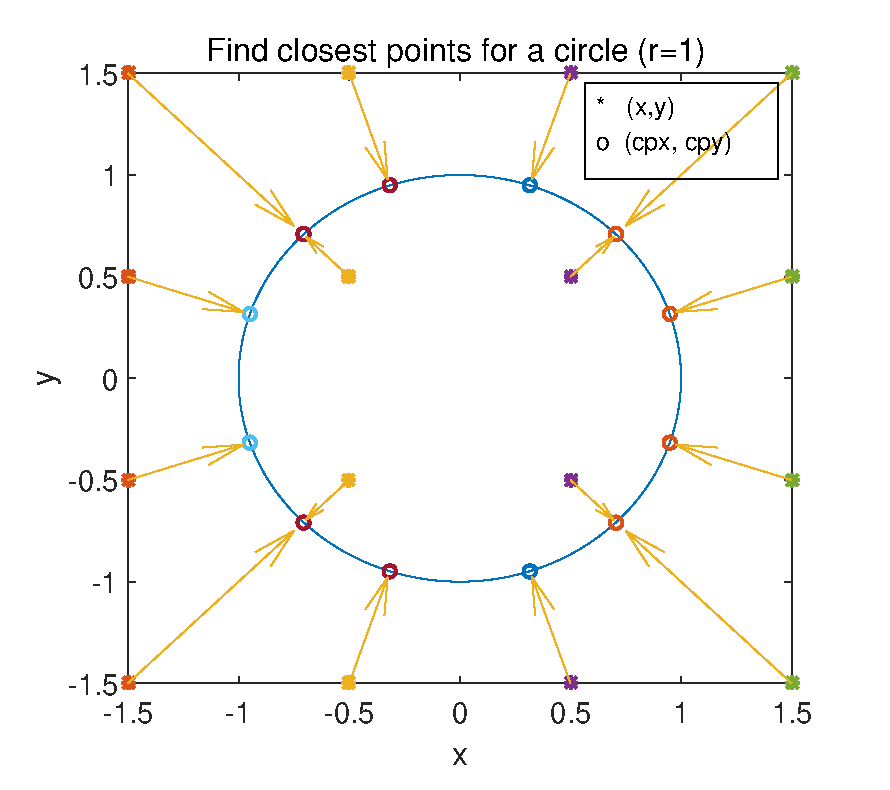
\includegraphics[width=0.5\textwidth]{UBC_IAM_5min_talk/Figures/Resultcp.eps}
        \end{figure}
    
\end{frame}

\begin{frame}{Closest Point Extension}
    Consider a function $u$ on the surface $S$, let $v$ be the value of the closest point on the function:
    $$v(\vec{x}) = u(cp(\vec{x}))$$
    \pause
    Thus, we can find the value by mapping $u(\vec{x})$ to $v(\vec{x})$.
    \newline
    \pause
    Define this operation as an operator $E$:
    $$v(\vec{x})=u(cp(\vec{x})) \Leftrightarrow v=Eu$$
\end{frame}

\begin{frame}{Closest Point principle}
    \begin{enumerate}
   \item <1-> Gradient Principle:
   $$\nabla(u(cp(\vec{x})))=\nabla_S u(\vec{x}),\ \vec{x}\in S$$\\
   \item <2-> Divergence Principle:
   $$\nabla\cdot(u(cp(\vec{x})))=\nabla_S \cdot u(\vec{x}),\ \vec{x}\in S$$
   \item <3->
   Then, we have the Laplace-Beltrami principle:
$$ \Delta u(cp(\vec{x}))=\Delta_S u(\vec{x}),\ \vec{x}\in S.$$
   \end{enumerate}

\end{frame}

\begin{frame}{Surface PDE to Extended PDE}
    A heat equation on the surface $S$:
    $$u_t=\Delta_S u$$
    \textbf{Solving steps:}
   \begin{enumerate}
   \item Using the Laplace-Beltrami principle:
   $$u_t=\Delta u(cp(\vec{x}))=\Delta Eu$$
   \item Apply the $E$ operator to both side:
   $$Eu_t=E\Delta Eu$$
   \item Static surface:
   $$(Eu)_t=E\Delta Eu \Leftrightarrow v_t = E\Delta v$$
   with constraint: $v = Ev$
   \item Discretize in time (Ruuth and Merriman, 2008):
   $$v^{n+1}=v^n+\Delta t(E\Delta v^n)$$
   \end{enumerate}
\end{frame}

\section{Radial Basis Function}

\begin{frame}{Radial Basis function}
    \alert{Radial basis functions $\phi(r)$} is a function that value only depends on the distance from the origin or the target data point if using on interpolation.
    
    There are different radial basis functions that can used depending on the problem:
    \begin{itemize}
        \item Infinite Smooth:
        \begin{itemize}
            \item Gaussian: $ e^{-\epsilon^{2}r^{2}}$
        \end{itemize}
        \item Piece-wise smooth:
        \begin{itemize}
            \item Polyharmonic Spline: $r^{2m-1}$ or $r^{2m}log(r)$ $m \in N$
        \end{itemize}
    \end{itemize}
    \pause
    To interpolate value:
    $$u(\vec{x}) = \sum_{j=1}^N \lambda_{j}\phi(r) = \sum_{j=1}^N\lambda_j\phi(|\vec{x}-\vec{x_j}||_2)$$
\end{frame}

\begin{frame}{Solving for weight}
    The coefficient $\lambda_j$ can be solved with the value of the function at the node $\vec{x_j}$. Impose that 
      $$
      u(\vec{x_i})  =     \sum_{j=1}^N\lambda_j\phi(||\vec{x_i}-\vec{x_j}||_2)\quad,
      \text{for } i = 1...N
      $$
      The number of N is the number of node point used to interpolate. Therfore, writing the system of equation in matrix:
      \pause
      $$
      \begin{pmatrix}
       \phi_{11} &\phi_{12}&\cdots &\phi_{1N}\\
       \phi_{21} &\phi_{22}& \cdots &\phi_{2N}\\
       \vdots &\vdots  &\cdots  & \vdots \\
       \phi_{N1} &\phi_{N2}& \cdots  &\phi_{NN}
     \end{pmatrix}\begin{pmatrix}\lambda_1\\ \lambda_2\\
     \vdots\\ \lambda_N\end{pmatrix}=\begin{pmatrix}u(x_1)\\ u(x_2)\\
     \vdots\\ u(x_N)\end{pmatrix},
     \phi_{ij}=\phi(\|\vec{x}_i-\vec{x}_j\|_2)
     $$
     $$A\vec{\lambda}=u(\vec{x_i})$$
     $$\vec{\lambda} = A^{-1}\vec{u}$$
\end{frame}

\begin{frame}{Interpolation}
    Recall from the original CPM
    $$
    v = Eu = u(cp(\vec{x}))
    $$
    Using RBF to interpolate the point \textbf{cp(x)} on the function u:
    $$
    u(cp(\vec{x}))  = \sum_{j=1}^N\lambda_j\phi(||cp(\vec{x})-x_j||_2)
    $$
    $$
    u(cp(\vec{x})) = 
    \begin{pmatrix}
    \phi(||cp(\vec{x})-x_1||_2) & \cdots & \phi(||cp(\vec{x})-x_N||_2)
    \end{pmatrix}
    \begin{pmatrix}
    \lambda_1 \\ \vdots \\ \lambda_N
    \end{pmatrix}
    $$
    $$
    u(cp\vec{x})) = C\vec{\lambda} =CA^{-1}\vec{u} = Eu
    $$
\end{frame}

\begin{frame}{RBF-FD}
    Laplacian can be discretized by RBF by simply applying the operator to the equation:
    $$ 
    \Delta u(\vec{x}) = \sum_{j=1}^N\lambda_j\Delta\phi(||\vec{x}-\vec{x_j}||_2)
    $$
    $$
    \begin{pmatrix}\Delta\phi(||\vec{x}-x_1||_2) &
    \cdots & \Delta\phi(||\vec{x}-x_N||_2)\end{pmatrix} 
    \begin{pmatrix}\lambda_1  \\ \vdots \\ \lambda_N\end{pmatrix} = \Delta u(\vec{x})
    $$
    $$B\vec{\lambda}=\Delta u$$
    $$BA^{-1}u=\Delta u$$
    $$\text{The laplacian operator is discretized as } \Delta = BA^{-1}$$
\end{frame}

\begin{frame}{Modification of RBF}
    Depends on the problem, there is a lot of modification can be made on RBF such as:
    \begin{itemize}
        \item \alert{Local method} (Flyer et al, 2016):
        \nextline Similar to the formation for all RBF matrix, but it constructed with the nearest m node instead of using all node.
        $$\text{mini }A = 
        \begin{pmatrix}
        \phi_{11}   & \cdots    & \phi_{1m} \\
        \vdots      & \ddots    & \vdots    \\
        \phi_{m1}   & \cdots    & \phi_{mm} \\
        \end{pmatrix}$$
        The resulting matrix will be extracted to place into the associate index of the node in a sparse matrix. The index of the nearest node can be obtained from the MAT-LAB built in function \textbf{knnsearch}.
    \end{itemize}
\end{frame}

\begin{frame}{Modification of RBF}
    Depends on the problem, there is a lot of modification can be made on RBF such as:
    \begin{itemize}
        \item \alert{Inclusion of polynomial term} (Flyer et al, 2016):
        \nextline The interpolating equation are constructed to include polynomial term in there
    $$ 
    u(\vec{x}) = \sum_{j=1}^N\lambda_j\phi(r) + \sum_{k=1}^K\gamma_k  p_k(\vec{x})
    $$
    with the constraints to maintain a square symmetric linear system and minimize far-field growth, $$\sum_{j=1}^N\lambda_j p_k(x_j) = 0,\quad k = 1,2...K$$
    
    \end{itemize}
\end{frame}

\begin{frame}{RBF-FD}
    \begin{figure}
      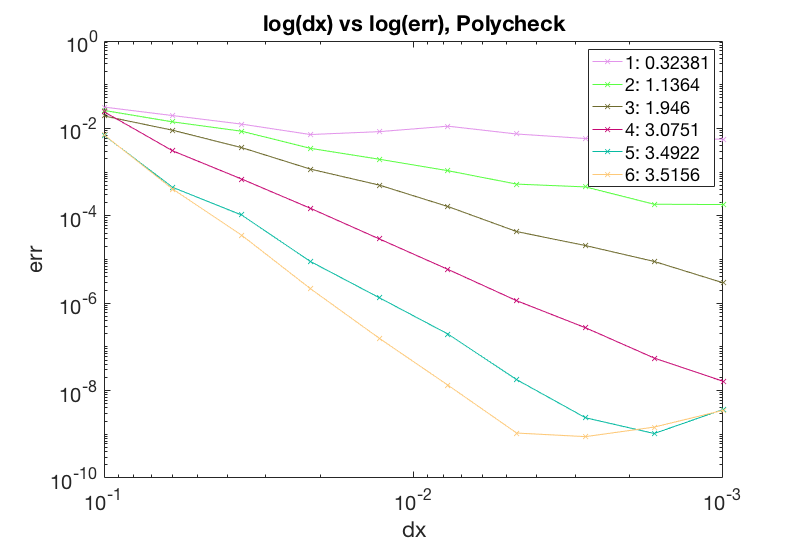
\includegraphics[width=0.7\textwidth]{UBC_IAM_5min_talk/Figures/RBF_FD.png}
      \caption{RBF-FD with different order of polynomial support}
    \end{figure}
\end{frame}

\begin{frame}{RBF-CPM}
    CPM is a method design to solve problem on surface:
    $$ 
    \Delta_s u = \pause \Delta Eu = \Delta u(cp(\vec{x})) \pause= \sum_{j=1}^N\lambda_j\Delta\phi(||cp(\vec{x)}-\vec{x_j}||_2)
    $$
    $$
    \begin{pmatrix}\Delta\phi(||cp(\vec{x})-x_1||_2) &
    \cdots & \Delta\phi(||cp(\vec{x})-x_N||_2)\end{pmatrix} 
    \begin{pmatrix}\lambda_1 \\ \vdots \\ \lambda_N\end{pmatrix} = \Delta u(cp(\vec{x}))
    $$
    $$\Tilde{B}\vec{\lambda}=\Delta u(cp(\vec{x}))$$
    $$\Tilde{B}A^{-1}u(\vec{x})=\Delta u(cp(\vec{x}))$$
    $$Du(\vec{x})=\Delta u(cp(\vec{x})) = \Delta Eu$$
    $$D:=\Delta E$$
\end{frame}

\section{Numerical example}

\begin{frame}{Heat equation on circle}
    \begin{columns}
    \column{0.5\textwidth}
        \begin{figure}
            \centering
            \begin{subfigure}
                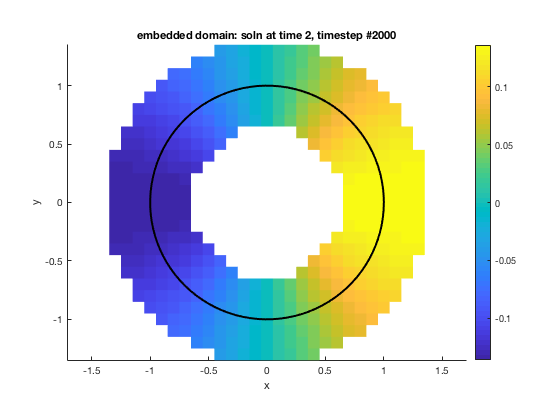
\includegraphics[width=1\textwidth]{UBC_IAM_5min_talk/Figures/heat_circle/heat_circle_CPM_plotdomain.png}
            \end{subfigure}
            \begin{subfigure}
                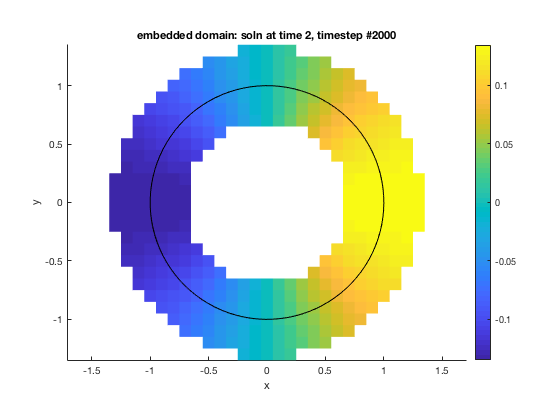
\includegraphics[width=1\textwidth]{UBC_IAM_5min_talk/Figures/heat_circle/heat_circle_RBFCPM_plotdomain.png}
            \end{subfigure}
        \end{figure}
    \pause
    \column{0.5\textwidth}
        \begin{table}[]
            \centering
            \begin{tabular}{c|c|c}
                 &  CPM & RBF-CPM\\
                 \hline \hline
                No.of point & 464 & 408 
            \end{tabular}
        \end{table}
    \end{columns}
\end{frame}

\begin{frame}{Heat equation on circle}
    \begin{figure}
        \centering
        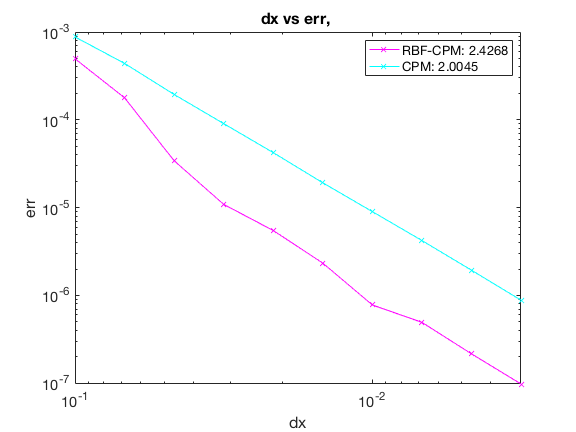
\includegraphics[width=0.7\textwidth]{UBC_IAM_5min_talk/Figures/heat_circle/heat_circle_RM_phs3_convergence_uniform_Polytermpt_skip_1_order_check.png}
        \caption{Convergence study of solving heat equation on circle via RBF-CPM and CPM}
    \end{figure}
\end{frame}

\begin{frame}{Heat equation on Sphere}
    \begin{columns}
    \column{0.5\textwidth}
        \begin{figure}
            \centering
            \begin{subfigure}
                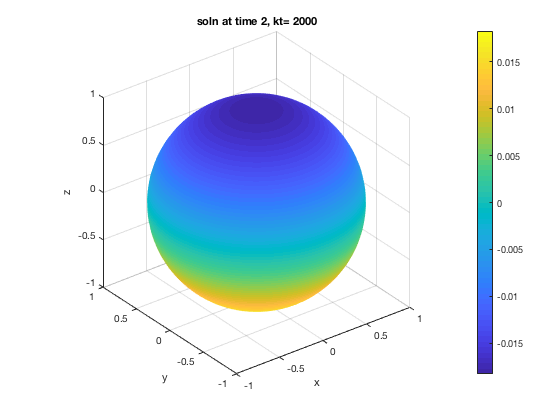
\includegraphics[width=1\textwidth]{UBC_IAM_5min_talk/Figures/heat_sphere/heat_sphere_CPM_plotdomain.png}
            \end{subfigure}
            \begin{subfigure}
                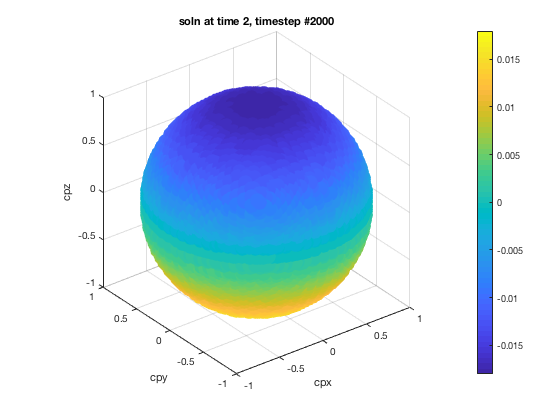
\includegraphics[width=1\textwidth]{UBC_IAM_5min_talk/Figures/heat_sphere/heat_sphere_RBFCPM_plotdomain.png}
            \end{subfigure}
        \end{figure}
    \pause
    \column{0.5\textwidth}
        \begin{table}[]
            \centering
            \begin{tabular}{c|c|c}
                 &  CPM & RBF-CPM\\
                 \hline \hline
                No.of point & 18922 & 6642
            \end{tabular}
        \end{table}
    \end{columns}
\end{frame}

\begin{frame}{Heat equation on Sphere}
    \begin{figure}
        \centering
        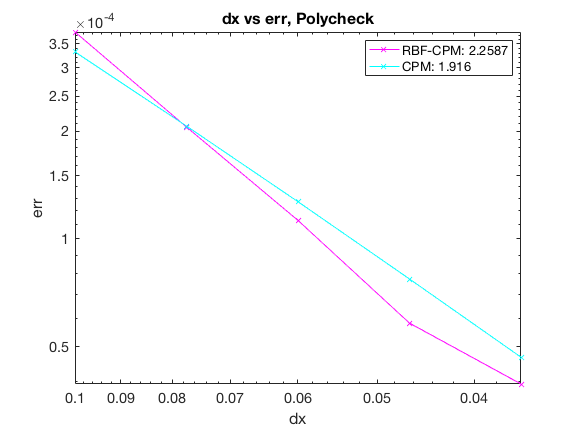
\includegraphics[width=0.7\textwidth]{UBC_IAM_5min_talk/Figures/heat_sphere/heat_sphere_RM_phs3_convergence_uniform_Polytermpt_skip_1_order_check.png}
        \caption{Convergence study of solving heat equation on sphere via RBF-CPM and CPM}
    \end{figure}
\end{frame}

\begin{frame}{Heat equation on Ellipse}
    \begin{columns}
    \column{0.5\textwidth}
        \begin{figure}
            \centering
            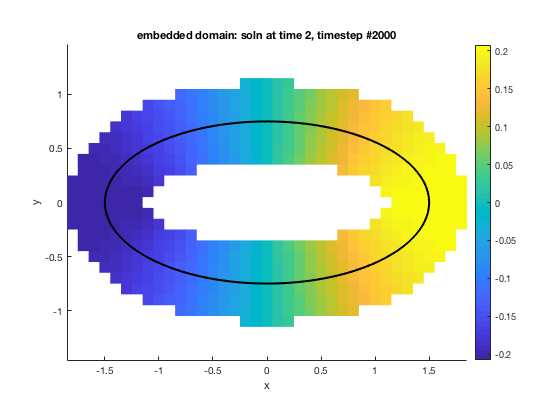
\includegraphics[width=1\textwidth]{UBC_IAM_5min_talk/Figures/heat_ellipse/heat_ellipse_CPM_plotdomain_a15b075.png}
            \caption{Solving heat on ellipse via CPM}
        \end{figure}
    \column{0.5\textwidth}
        \begin{figure}
            \centering
            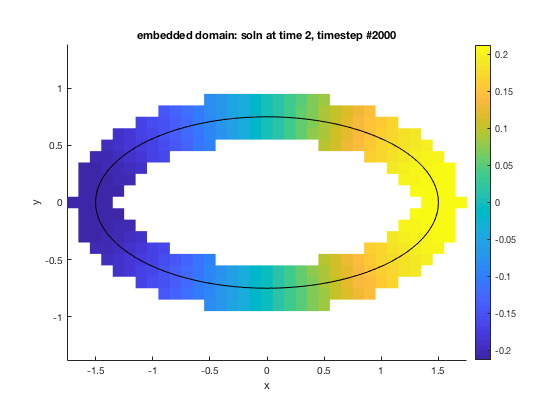
\includegraphics[width=1\textwidth]{UBC_IAM_5min_talk/Figures/heat_ellipse/heat_ellipse_RBFCPM_plotdomain_a15b075.png}
            \caption{Solving heat on ellipse via RBF-CPM}
        \end{figure}
    \end{columns}
\end{frame}

\begin{frame}{Heat equation on thin Ellipse}
    \pause
    \begin{columns}
    \column{0.5\textwidth}
        \begin{figure}
            \centering
            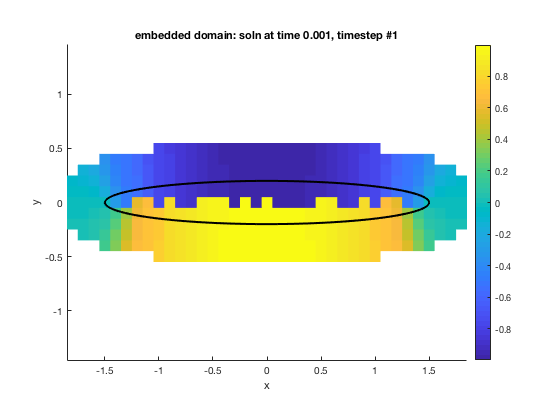
\includegraphics[width=1\textwidth]{UBC_IAM_5min_talk/Figures/heat_ellipse/heat_ellipse_CPM_plotdomain_a15b02_init.png}
            \caption{Solution for heat on thin ellipse at time 0.001}
        \end{figure}
    \column{0.5\textwidth}
        \begin{figure}
            \centering
            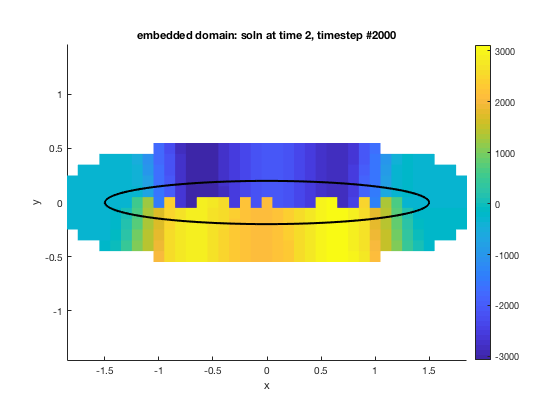
\includegraphics[width=1\textwidth]{UBC_IAM_5min_talk/Figures/heat_ellipse/heat_ellipse_CPM_plotdomain_a15b02.png}
            \caption{Solution for heat on thin ellipse at time 2}
        \end{figure}
    \end{columns}
\end{frame}

\begin{frame}{Heat equation on thin Ellipse}
    To solve this problem, CPM require a refined mesh around the ellipse so that their computational grid will not cross with the grid of the other side of the ellipse
    \begin{columns}
    \column{0.5\textwidth}
        \begin{figure}
            \centering
            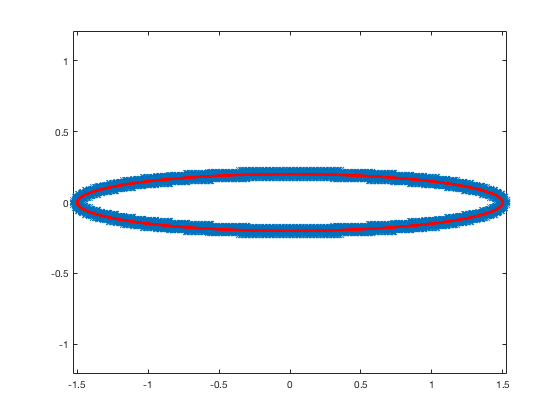
\includegraphics[width=1\textwidth]{UBC_IAM_5min_talk/Figures/heat_ellipse/heat_ellipse_CPM_refinedgrid.png}
        \end{figure}
        \pause
    \column{0.5\textwidth}
        \begin{figure}
            \centering
            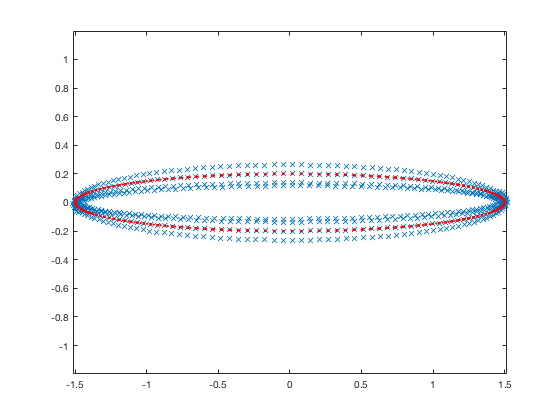
\includegraphics[width=1\textwidth]{UBC_IAM_5min_talk/Figures/heat_ellipse/heat_ellipse_RBFCPM_ellipticgrid.png}
        \end{figure}
    \end{columns}
\end{frame}

\begin{frame}{Heat equation on thin Ellipse}
    \begin{figure}
      \begin{subfigure}
        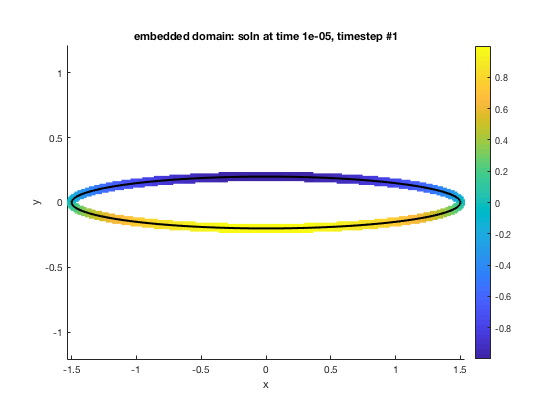
\includegraphics[width=0.45\textwidth]{UBC_IAM_5min_talk/Figures/heat_ellipse/heat_ellipse_CPM__refined_plotdomain_a15b02_init.png}
      \end{subfigure}
      \begin{subfigure}
        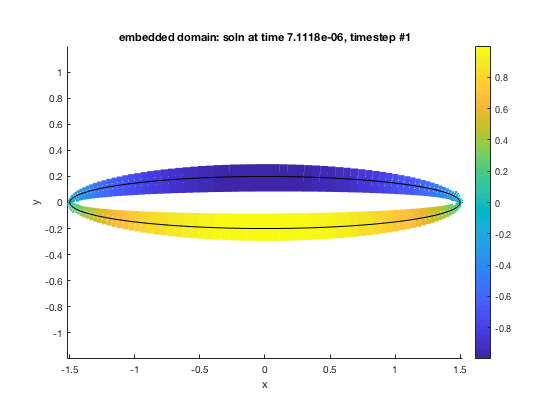
\includegraphics[width=0.45\textwidth]{UBC_IAM_5min_talk/Figures/heat_ellipse/heat_ellipse_RBFCPM__elliptic_plotdomain_a15b02_init.png}
      \end{subfigure}
      \begin{subfigure}
        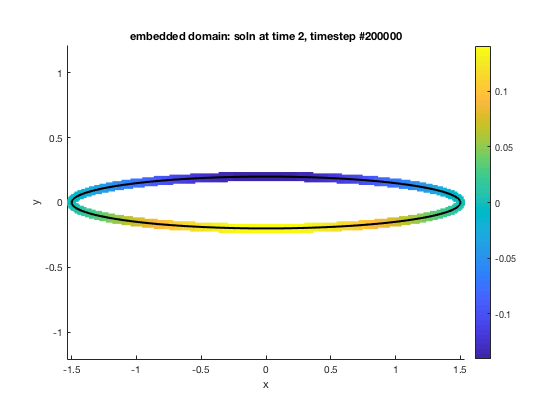
\includegraphics[width=0.45\textwidth]{UBC_IAM_5min_talk/Figures/heat_ellipse/heat_ellipse_CPM__refined_plotdomain_a15b02.png}
      \end{subfigure}
      \begin{subfigure}
        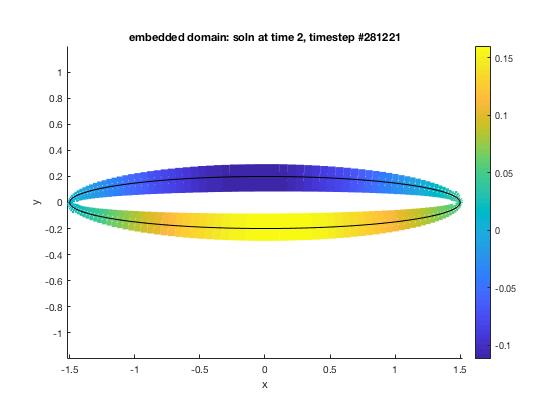
\includegraphics[width=0.45\textwidth]{UBC_IAM_5min_talk/Figures/heat_ellipse/heat_ellipse_RBFCPM__elliptic_plotdomain_a15b02.png}
      \end{subfigure}
    \end{figure}
\end{frame}

\begin{frame}{Heat equation on thin Ellipse}
    \begin{columns}
    \column{0.5\textwidth}
        \begin{figure}
            \centering
            \begin{subfigure}
                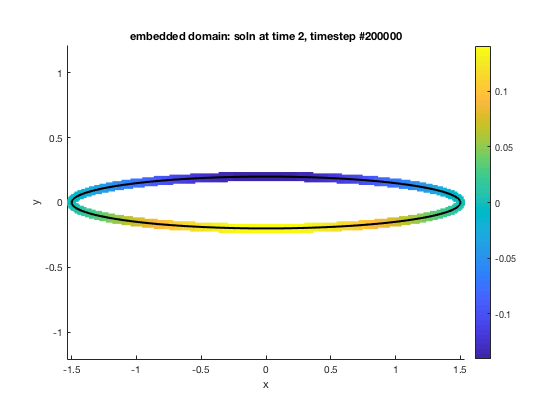
\includegraphics[width=1\textwidth]{UBC_IAM_5min_talk/Figures/heat_ellipse/heat_ellipse_CPM__refined_plotdomain_a15b02.png}
            \end{subfigure}
            \begin{subfigure}
                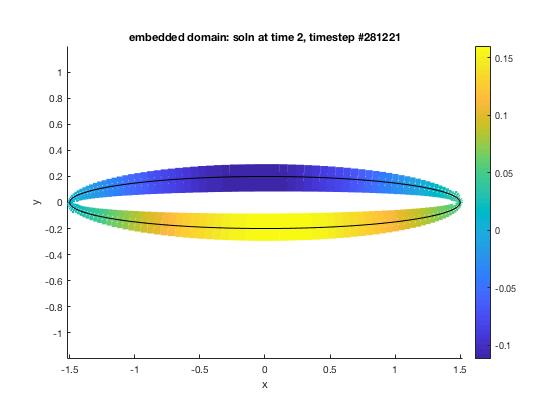
\includegraphics[width=1\textwidth]{UBC_IAM_5min_talk/Figures/heat_ellipse/heat_ellipse_RBFCPM__elliptic_plotdomain_a15b02.png}
            \end{subfigure}
        \end{figure}
    \pause
    \column{0.5\textwidth}
        \begin{table}[]
            \centering
            \begin{tabular}{c|c|c}
                 &  CPM & RBF-CPM\\
                 \hline \hline
                No.of point & 4424 & 615
            \end{tabular}
        \end{table}
    \end{columns}
\end{frame}

\section{Summary and future work}

\begin{frame}{Comparison between CPM and RBF-CPM}
    By comparing the solution of solving heat equation on circle, sphere, ellipse via the original CPM method and the new combined method,
    \begin{itemize}
        \item <1-> Accuracy
        \item <2-> Rate of convergence
        \item <3-> Flexibility
        \item <4-> Grid size
                    \begin{table}[]
                        \centering
                        \begin{tabular}{c|c|c}
                              &  CPM & RBF-CPM\\
                             \hline \hline
                            Circle & 464 & 408\\
                            Ellipse & 526 & 296\\
                            Sphere & 18922 & 6642\\
                            Thin Ellipse & 4424 & 615\\
                        \end{tabular}
                    \end{table}
    \end{itemize}
\end{frame}

\begin{frame}{Future Work}
    \begin{figure}
      \begin{subfigure}
        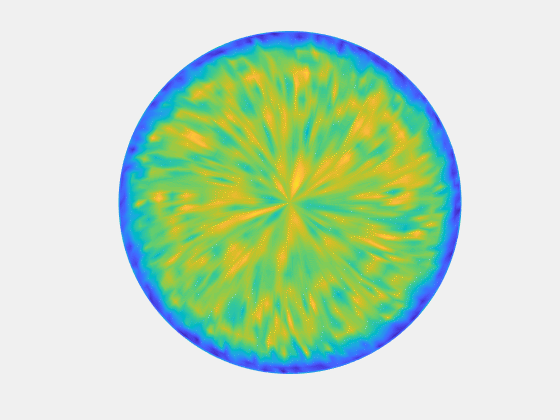
\includegraphics[width=0.45\textwidth]{UBC_IAM_5min_talk/Figures/animatedgif/frame1.png}
       \end{subfigure}
       \begin{subfigure}
        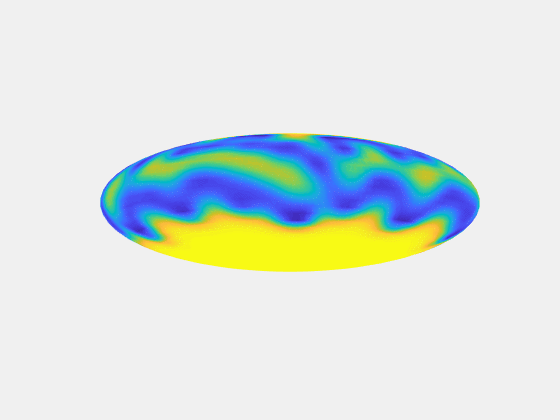
\includegraphics[width=0.45\textwidth]{UBC_IAM_5min_talk/Figures/animatedgif/frame100.png}
        \end{subfigure}
        \begin{subfigure}
        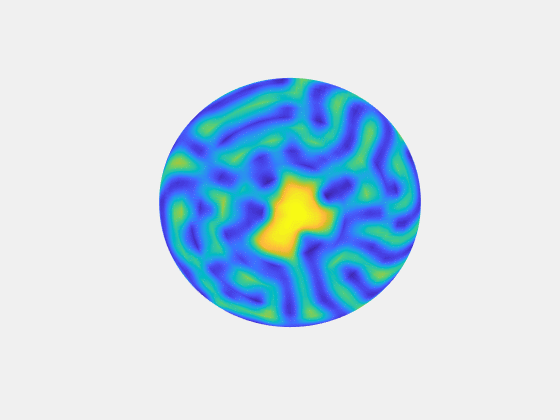
\includegraphics[width=0.45\textwidth]{UBC_IAM_5min_talk/Figures/animatedgif/frame200.png}
        \end{subfigure}
        \begin{subfigure}
        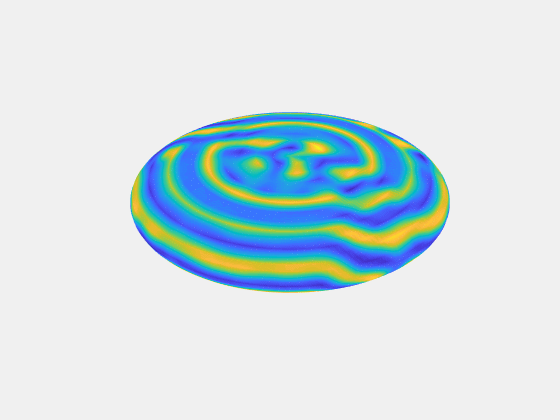
\includegraphics[width=0.45\textwidth]{UBC_IAM_5min_talk/Figures/animatedgif/frame300.png}
      \end{subfigure}
    \end{figure}
\end{frame}

\begin{frame}{Acknowledgement}
    \centering
    % \animategraphics[autoplay,controls,width=\linewidth]{1}{UBC_IAM_5min_talk/Figures/animated gif/frame}{1}{200}
    \textbf{Thank you to Professor Colin B. Macdonald and Tony Wong !} 
\end{frame}

\end{document}